% !TEX root = /home/eb/.vscode/extensions/qftrules.programme-colle/tmp/Exercice.tex



\begin{exo}[PC][1][exp]{Échelle de perroquet}
  \Notions{\item Onde mécanique \task Régime libre \task TMC}
Une échelle de perroquet constituée de barreaux tous identiques, de moment d'inertie $J$ par rapport à leur axe vertical de rotation $(Ox)$, est suspendue au plafond. Les barreaux sont liés deux à deux par des fils de torsion, de longueur $a$ et de constante de raideur $C$. On note $\theta_n$ l’angle du $n^{\text{e}}$ barreau par rapport à sa position d'équilibre.
%\begin{figure}[h!]
%\centering
\begin{center}
% 
\includegraphics[width=0.135\textwidth]{echelle_perroquet.png}\qquad

\includegraphics[width=0.25\textwidth]{perroquet.pdf}
\end{center}
%\end{figure}
\begin{quest}
  \item En appliquant le TMC au barreau numéro $n$, montrer que 
  % $$
  \begin{equation}
    \ddot{\theta}_n = \omega_0^2\,(\theta_{n+1}+\theta_{n-1}- 2\theta_n),
  \end{equation}
  où $\omega_0 $ est une constante à exprimer en fonction de $C$ et $J$.
  % $$
  \sol{
    \udl{Référentiel} : laboratoire, supposé galiléen.


    \udl{Système} : barreau $n$, angle $\theta_n$, moment d’inertie $J$, moment cinétique $\Vec{L}_n= J \dot{\theta}_n \ez $.

    \udl{Bilan des actions mécaniques} : moments $\Vec{\Gamma}_{n+1} = C(\theta_{n+1}-\theta_n)\ez$  et $\Vec{\Gamma}_{n+1} = C(\theta_{n}-\theta_{n-1})\ez$

\udl{TMC} :
$$
\dd{\Vec{L}}{t} = J \ddot{\theta_n} \ez = \Vec{\Gamma}_{n+1} + \Vec{\Gamma}_{n} \Rar J \ddot{\theta_n} = C(\theta_{n+1}-\theta_n)  + C(\theta_{n}-\theta_{n-1}) = C(\theta_{n+1} + \theta_{n-1} - 2 \theta_{n}).
$$
donc
% $$
\eqbox{
  \ddot{\theta_n} = \frac{C}{J}(\theta_{n+1} + \theta_{n-1} - 2 \theta_{n}).
  }
% $$
  }
\item À quelle condition l’approximation du continu est-elle valable ?
 Montrer que l'équation de propagation d'une onde de torsion le long de l'échelle s’écrit 
%  \eqbox{
  \begin{equation}
    \ddr{\theta}{x} - \frac{1}{c^2}\ddr{\theta}{t}=0. 
  \end{equation}
%  }
 Quelle est l’expression de la célérité $c$ en fonction de $a$, $C$ et $J$ ?
\sol{
\udl{Approximation du continu} :
On suppose la longueur d’onde $\lambda \gg a$, et on remplace $\theta_n(t)$ par une fonction lisse $\theta(x,t)$. Par Taylor,
$$
\theta_{n+1} + \theta_{n-1} - 2 \theta_{n} \simeq  a^2 \ddr{\theta}{x}.
$$
donc
$$
\ddr{\theta}{x} - \frac{J}{Ca^2} \ddr{\theta}{t} = 0.
$$
C’est une équation de D’Alembert avec $c=\sqrt{\frac{Ca^2}{J}}$. $C$ représente une \guill{tension} et $J$ une \guill{inertie}.
}
% \item Que devient-elle dans l'approximation des milieux continus ? Déterminer la valeur du ou des paramètres de l'équation d'onde en fonction des caractéristiques de l'échelle.
% \sol{
% On suppose la longueur d’onde $\lambda \gg a$, et on remplace $\theta_n(t)$ par une fonction lisse $\theta(x,t)$. Par Taylor,
% $$
% \theta_{n+1} + \theta_{n-1} - 2 \theta_{n} \simeq  a^2 \ddr{\theta}{x}.
% $$
% donc
% $$
% \ddr{\theta}{x} - \frac{J}{Ca^2} \ddr{\theta}{t} = 0.
% $$
% C’est une équation de D’Alembert avec $c=\sqrt{\frac{Ca^2}{J}}$. $C$ représente une \guill{tension} et $J$ une \guill{inertie}.
% }
\end{quest}
Pour visualiser la propagation, voir par exemple \url{https://youtu.be/boshutQYCbk}, ou l’expérience de cours.
\end{exo}
%%%%%%%%%%%%%%%%%%%%%%%%%%%%%%%%%%%%%%%%%%%%%%%%%%%

%%%%%%%%%%%%%%%%%%%%%%%%%%%%%%%%%%%
\begin{exo}[PC][3][TD]{Spectre d’une corde de piano et de clavecin}
  % \Annale[Physique PC]{E3A}{2022}
  \Notions{\item Onde mécanique \item Série de Fourier \task Modes propres}
  Une corde de clavecin de longueur $L$ est pincée en son milieu pour produire un son. En première approximation, la corde a, à l’instant initial, le profil d’un triangle isocèle de hauteur $a$ au milieu, comme sur la \Fig{clavecin}. On cherche une solution sous la forme d’une série de Fourier, i.e. d’une superposition de modes propres. À une origine des temps près, on pose donc
  \begin{equation}
    y(x,t) = \sum_{n =0}^{\infty} A_n \sin\left(n\pi \frac{x}{L}\right) \cos\left(n\pi \frac{ct}{L}\right).
  \end{equation}


    %\capt{}
\begin{quest}
  \item	Vérifier que la fonction définie satisfait aux conditions aux limites en $x=0$ et $x=L$.
  \sol{
    On a bien
    $$
  y(x=0,t) = \sum_{0}^{\infty} A_n \sin(0)  \cos\left(n\pi \frac{ct}{L}\right) = 0,
    $$
    et 
    $$
y(x=L,t) =  \sum_{0}^{\infty} A_n \sin(n\pi)  \cos\left(n\pi \frac{ct}{L}\right) = 0.
    $$
  }
  \item On admet que les coefficients de Fourier $A_n$, avec $n\in \N$, s’obtiennent par la relation 
  \begin{equation}
    A_n = \frac{2}{L}\int_0^L y(x,t = 0)\sin\left(n\pi \frac{x}{L}\right) \d x. 
  \end{equation}
  Exprimer analytiquement la fonction $y(x,t=0)$ pour le clavecin, puis déterminer les coefficients $A_n$. 

  \sol{
    La fonction $y(x,t=0)$ s’écrit 
    $$
    y(x,t=0) = \frac{2b}{L}x~(0<x<L/2), \qquad y(x,t=0) = \frac{2b}{L}(L-x)~(L/2<x<L).
    $$
    On a donc 
    $$
  A_n = \int_0^{L/2} \frac{4b}{L^2}x \sin\left(n\pi \frac{x}{L}\right) \d x + \int_{L/2}^L \frac{4b}{L^2}(L-x) \sin\left(n\pi \frac{x}{L}\right) \d x  = \int_0^{L/2} \frac{4b}{L^2}x \sin\left(n\pi \frac{x}{L}\right) \d x + \int_{0}^{L/2} \frac{4b}{L^2}u \sin\left(n\pi -n\pi \frac{u}{L}\right) \d u ,
    $$
    soit 
    $$
    A_n = \frac{4b}{L^2} [1+(-1)^{n+1}] I_n, \qquad I_n = \int_0^{L/2} x \sin\left(n\pi \frac{x}{L}\right) \d x.
    $$
    Le coefficient de Fourier est donc nul si $n$ est pair. Si $n=2m+1$ est impair, le coefficient vaut 
    $$
  A_{2m + 1} = \frac{8a}{L^2} I_{2m+1},
$$
    œu l’intégrale se calcule par intégration par parties,
    % $$
    \begin{equation*}
      \begin{split}
        I_{2m + 1} = \left[ -\frac{xL}{(2m +1)\pi} \cos\left(n\pi \frac{x}{L}\right) \right]_{0}^{L/2} + \frac{L}{(2m + 1)\pi} \int_0^{L/2} \cos\left(n\pi \frac{x}{L}\right) \d x\\
        = \frac{L^2}{(2m +1)\pi} \cos(\pi / 2)+ \frac{L^2}{(2m + 1)^2\pi^2} \left[ \sin(n\pi \frac{x}{L}) \right]_0^{L/{2}} \\ = 
         \frac{L^2}{(2m + 1)^2\pi^2}.
      \end{split}
      \end{equation*}
      On en déduit 
      \eqbox{
      A_{n} = \frac{8a}{\pi^2}\frac{1}{n^2}.
      }
      si  $n$ impair, et $A_n = 0$  sinon.
    % $$
  }
  \item On rappelle que la densité linéique d’énergie s’écrit
  \begin{equation}
    e = \frac{1}{2} \mu \left( \dr{y}{x} \right)^2 + \frac{1}{2} T \left( \dr{y}{t} \right)^2.
  \end{equation}
  Calculer l’énergie $E_n$ dans chaque mode, ainsi que l’énergie totale $E$. Représenter le spectre de Fourier, i.e. le  spectre énergétique en fréquence.
  \item Reprendre les calculs précédents pour une corde de piano, qui est frappée par un marteau de vitesse~$v_0$ entre les abscisses $x=0$ et $x=b$. En particulier, préciser les conditions initiales, calculer les coefficients $A_n$, représenter le spectre de Fourier, et déterminer l’énergie totale $E$.
  % La condition initiale s’écrit alors 
  % \begin{equation}
  %   % \begin{align}{ll}
  %     \dr{y}{t}(x,t = 0) = v_0 ~(0 <x < b),    \qquad   \dr{y}{t}(x,t = 0) = 0~(b < x < L). 
  %   % \end{align}
  % \end{equation}
\end{quest}

  \begin{fig}[label]
    \centering
    \begin{subfig}[clavecin][0.45]
      
\includegraphics[width=\columnwidth]{clavecin.pdf}
    \end{subfig}\hspace{0.5cm}
        \begin{subfig}[label][0.45]
      
\includegraphics[width=\columnwidth]{piano.pdf}
    \end{subfig}
  \end{fig}
\capt{(a) Corde de clavecin. (b) Corde de piano.}
\end{exo}
%%%%%%%%%%%%%%%%%%%%%%%%%%%%%%%%%%%

%%%%%%%%%%%%%%%%%%%%%%%%%%%%%%%%%%%%%%%%%%%%%%%%%%%
\begin{exo}[PC][1][TD]{Modes propres d'une chaîne de systèmes masse-ressort couplés}
On considère un système de $N$ masses $m$, couplées par des ressorts identiques de longueur à vide $l_0$ et de constante de raideur $k$. À la fin de chaque question il est conseillé de visualiser l'animation suivante pour vérifier ses résultats et bien comprendre ce qu'il se passe: \url{http://ressources.univ-lemans.fr/AccesLibre/UM/Pedago/physique/02/meca/chaine.html}.
\begin{quest}
\item On étudie dans un premier temps en détail le cas $N=2$ représenté ci-dessous.
%\begin{figure}[h!]
%\centering
\begin{center}

\includegraphics[width=0.6\columnwidth]{chaine_N=2.pdf}
\end{center}
%\end{figure}
\begin{enumerate}
\item Établir le système d'équations couplées caractérisant le mouvement.

\item Résoudre le système précédent et déterminer les modes propres et les pulsations propres associées. Déterminer ensuite l'expression des allongements $\xi_1(t)$ et $\xi_2(t)$. Montrer qu'en supposant que $\xi_1(0)\neq 0$ et $\xi_2(0)=0$ et de plus ${\xi}_1(0)=0={\xi}_2(0)$ (absence de vitesse initiale) on obtient
\begin{equation}
\begin{cases}
\xi_1(t)=\frac{1}{2}\xi_1(0)\left[\cos(\omega_0 t)+\cos(\sqrt{3}\omega_0 t)\right],\\[1mm]
\xi_2(t)=\frac{1}{2}\xi_1(0)\left[\cos(\omega_0 t)-\cos(\sqrt{3}\omega_0 t)\right]. \end{cases}
\end{equation}

\item Montrer que les modes propres et les pulsations propres sont en fait simplement reliés aux vecteurs propres et aux valeurs propres d'une matrice $M\in\mc{M}_{2}(\mathbb{R})$ symétrique (et donc diagonalisable et à valeurs propres réelles) telle que
\begin{align}
    \frac{\der^2}{\der t^2}\begin{bmatrix}
           \xi_1 \\
           \xi_2
         \end{bmatrix} &= M \begin{bmatrix}
           \xi_1 \\
           \xi_2
         \end{bmatrix}.
         \end{align}
Interpréter ces modes propres en termes de mouvements des masses couplées sur un schéma.
\end{enumerate}
\item En s'inspirant de la méthode précédente, expliquer sans terminer explicitement les calculs comment il faudrait faire pour résoudre le cas $N=3$.
\item On souhaite maintenant étudier le cas général de $N$ masses couplées.
\begin{enumerate}
\item Justifier que l'équation vérifiée par la masse couplée numéro $n$ est de la forme 
\begin{equation}
  \frac{\der^2\xi_{n}}{\der t^2}=\omega_0^2(\xi_{n+1}+\xi_{n-1}-2\xi_{n}).
\end{equation}
\item En cherchant une solution sous la forme complexe $\underline{\xi}_n = A\,\e^{i(\omega t-kna)}$ où $a$ est la distance entre deux masses voisines au repos, montrer que la relation de dispersion des ondes dans la chaîne se met sous la forme $\omega^2=4\omega_0^2\sin^{2}(\frac{ka}{2})$.
\item Que se passe-t-il dans le cas où $ka\ll 1$ ? Commenter.
\end{enumerate}
\end{quest}
\end{exo}
%%%%%%%%%%%%%%%%%%%%%%%%%%%%%%%%%%%%%%%%%%%%%%%%%%%

%%%%%%%%%%%%%%%%%%%%%%%%%%%%%%%%%%%%%%%%%%%%%%%%%%%
\begin{exo}[PC]{Ondes et musique: la guitare}
En musique, le doublement de la fréquence d'un son correspond à ce que l'on appelle un changement d'octave. La gamme dite tempérée (la plus simple et la plus utilisée) divise l'octave en 12 intervalles égaux appelés demi-tons. Les fréquences successives des notes espacées par ces demi-tons forment une suite géométrique telle que $f_{p}=2^{\frac{p}{12}}f$ où $p\in[1;12]$. Le même demi-ton sonne de façon similaire à l'oreille quel que soit l'octave: on lui attribue donc un nom (do, do$\sharp$, ré, ré$\sharp$, mi, fa, fa$\sharp$, sol, sol$\sharp$, la, la$\sharp$, si, do ...). La base de fréquence de la gamme tempérée est le $la_3$ (la de la $3^{\rm{ème}}$ octave) à \SI{440}{Hz}. Le savart (unité associée au pouvoir séparateur de l'oreille) permet de quantifier l'écart de hauteur entre deux sons: deux fréquences $f_1$ et $f_2$ sont séparées de $1000\times\log\left(\frac{f_1}{f_2}\right)$ savarts.
\begin{quest}
\item Les fréquences fondamentales des cordes d'une guitare sont $[mi_1;la_1;ré_2;sol_2;si_2;mi_3]$. Déterminer la fréquence correspondant à chaque corde.
\item Les cordes d'une guitare électrique sont faites d'acier de masse volumique $\rho=\SI{7,8e3}{}$ $\SI{}{kg.m^{-3}}$ et leurs diamètres respectifs en \SI{}{mm} sont $[1,12;0,89;0,70;0,55;0,35;0,25]$. En supposant que la longueur de chaque corde vaut \SI{63}{cm}, déterminer les tensions nécessaires pour que la guitare soit parfaitement accordée.
\item Quelle est la variation relative qui peut être tolérée sur la tension de la quatrième corde ($sol_2$) pour que la fréquence du fondamental correspondant ne varie pas de plus de 5 savarts (limite de séparation de l'oreille moyenne) ?
\item De combien doit-on déplacer son doigt toujours sur la corde 4 pour passer du $sol_2$ au $la_2$ ? Commenter.
%\item On rappelle que la forme générale des oscillations libres d'une corde vibrante fixée à ses deux extrémités se met sous la forme
%\begin{equation}
% s_{n}(x,t)=\sum_{n=1}^{\infty}\left[\bigg\{A_{n}\cos(n\omega_{0}t)+B_n\sin(n\omega_0 t)\bigg\}\sin\left(\frac{n\omega_0 x}{c}\right)\right]
% \end{equation}
% On peut montrer que les coefficients $A_n$ et $B_n$ (appelés coefficients de Fourier) s'obtiennent à partir des conditions initiales en évaluant les intégrales suivantes
% \begin{equation}
% \begin{split}
%A_n&=\frac{1}{L}\int_{-L}^{L}\sin(\frac{n\pi x}{L})s(x,0)\,\derer x \\
%B_n&=\frac{1}{n\pi c}\int_{-L}^{L}\sin(\frac{n\pi x}{L})\frac{\partial s}{\partial t}(x,0)\,\derer x \\
%\end{split}
% \end{equation}
% Lors du pincement de la corde, on considère que celle-ci est abandonnée sans vitesse initiale depuis la forme représentée ci-dessous.
%
% \begin{figure}[h!]
% \centering
% 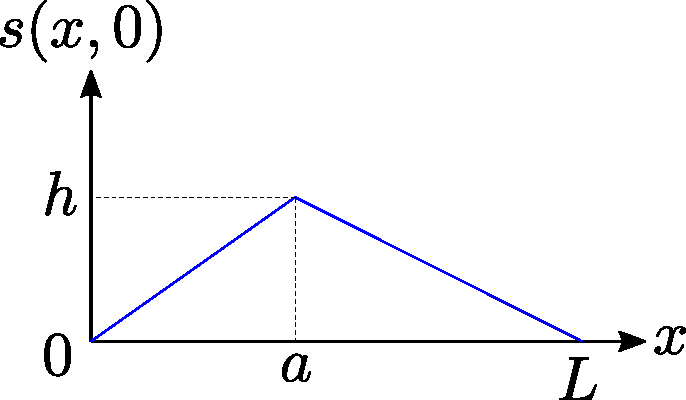
\includegraphics[width=0.3\textwidth]{Figures/corde_pincée.pdf}
% \end{figure}
%
%\begin{enumerate}
%\item Calculer les amplitudes des différents harmoniques présents dans la corde.
%\item Montrer qu'en pinçant la corde en un point d'abscisse $a$ bien choisi, le premier harmonique dissonant ($n=7$) peut être supprimé.
%\end{enumerate}
\end{quest}
\end{exo}
%%%%%%%%%%%%%%%%%%%%%%%%%%%%%%%%%%%%%%%%%%%%%%%%%%%
%

%%%%%%%%%%%%%%%%%%%%%%%%%%%%%%%%%%%
\begin{exo}[PC][2][TD]{Étude énergétique d'une corde vibrante}
  \Notions{\item Énergie \task Corde vibrante \task OPP \task Mode propre}
On considère une corde sans raideur attachée à ces deux extrémités $x=0$ et $x=L$ et soumise à une tension $T$. Sa masse linéique est constante te vaut $\mu$. Un point de cette corde au repos à l'abscisse~$x$ est à la cote $y=0$ ; en mouvement, sa cote devient $y(x, t)$. On suppose l'angle de courbure $\alpha(x,t) \ll 1$.
\begin{quest}
  \item Montrer que la densité linéique d'énergie cinétique a pour expression 
  \begin{equation}
    e_c = \frac{1}{2} \mu \left( \dr{y}{t} \right)^2.
  \end{equation}
  \item Montrer de même que l’on peut définir une densité linéique d'énergie potentielle, d'expression
  \begin{equation}
e_p=\frac{T}{2}\left( \dr{y}{x} \right)^2.
  \end{equation}
 Montrer que  $e_c=e_p$ pour une onde plane progressive.
  \item On considère un mode propre de la corde: $y_n(x, t)=A_n \sin \left(\omega_n t+\varphi_n\right) \sin \left(k_n x\right)$ avec $k_n=n \pi / L$ et $\omega_n = c k_n$. Calculer l'énergie totale $E_n$ de la corde en fonction de $A_n, n, L$ et $T$.
  % \item Calculer l'énergie totale $E$ d'une corde attachée à ces deux extrémités; on montrera, puisque $\int_0^l \sin \left(k_p x\right) \sin \left(k_q x\right) \mathrm{d} x=\frac{1}{2} l \delta_{p, q}$ (de même pour les cosinus), que $E=\sum_{n=1}^{\infty} E_n$.
\end{quest}
\end{exo}
%%%%%%%%%%%%%%%%%%%%%%%%%%%%%%%%%%%

%%%%%%%%%%%%%%%%%%%%%%%%%%%%%%%%%%%%%%%%%%%%%%%%%%%%%%%%%
\begin{exo}[PC][3][TD]{Modes propres d'une chaîne de systèmes masse-ressort}
  \Notions{\item Onde mécanique \task Onde longitudinale \task Mode propre}
On considère un système de $N$ masselottes de masse $m$, couplées par des ressorts identiques de longueur à vide $\ell_0$ et de constante de raideur $k$. À la fin de chaque question il est conseillé de visualiser l'animation suivante pour vérifier ses résultats et bien comprendre ce qu'il se passe: \url{http://ressources.univ-lemans.fr/AccesLibre/UM/Pedago/physique/02/meca/chaine.html}.
\begin{quest}
\item On étudie dans un premier temps en détail le cas $N=2$ représenté ci-dessous.
%\begin{figure}[h!]
%\centering
\begin{center}

\includegraphics[width=0.6\columnwidth]{chaine_N=2.pdf}
\end{center}
%\end{figure}
\begin{enumerate}
\item Établir le système d'équations couplées caractérisant le mouvement.
\sol{
Voir  cours. Ici, les positions $x_0$ et $x_3$ des bords sont fixes. On a donc
$$
\begin{cases}
  \dd{\xi_1}{t} & = \frac{k}{m}(\xi_2-2\xi_1) \\
  \dd{\xi_2}{t} & = \frac{k}{m}(\xi_1-2\xi_2) \\
\end{cases}
$$
}
\item Résoudre le système précédent et déterminer les modes propres et les pulsations propres associées. Déterminer ensuite l'expression des allongements $\xi_1(t)$ et $\xi_2(t)$. Montrer qu'en supposant que $\xi_1(0)\neq 0$ et $\xi_2(0)=0$ et de plus $\frac{\der{\xi}_1}{\der t}(0)=0=\frac{\der{\xi}_2}{\der t}(0)$ (absence de vitesse initiale) on obtient
\begin{equation}
\begin{cases}
\xi_1(t)=\frac{1}{2}\xi_1(0)\left[\cos(\omega_0 t)+\cos(\sqrt{3}\,\omega_0 t)\right],\\[1mm]
\xi_2(t)=\frac{1}{2}\xi_1(0)\left[\cos(\omega_0 t)-\cos(\sqrt{3}\,\omega_0 t)\right]. \end{cases}
\end{equation}
\sol{
On pose $\xi_+ = \xi_1 + \xi_2$ et $\xi_- = \xi_1 - \xi_2$, puis on somme ou retranche les deux équations pour trouver
$$
\begin{cases}
  \dd{\xi_+}{t} & = -\frac{k}{m}\xi_+ \\
  \dd{\xi_-}{t} & = -\frac{3k}{m}\xi_- \\
\end{cases}
$$
On obtient deux modes propres:
$$
\begin{cases}
  \xi_+(t) & = A \cos(\omega_+ t) \\
  \xi_-(t) & = A \cos(\omega_- t)\\
\end{cases}
$$
avec $\omega_+ = \sqrt{\frac{k}{m}}$ et $\omega_- =  \sqrt{\frac{3k}{m}}$.
}
\item Montrer que les modes propres et les pulsations propres sont en fait simplement reliés aux vecteurs propres et aux valeurs propres d'une matrice $M\in\mc{M}_{2}(\mathbb{R})$ symétrique réelle (et donc diagonalisable et à valeurs propres réelles) telle que
\begin{align}
   \frac{\der^2}{\der t^2}\begin{pmatrix}
          \xi_1 \\
          \xi_2
        \end{pmatrix} + M\omega_0^2 \begin{pmatrix}
          \xi_1 \\
          \xi_2
        \end{pmatrix}=0.
        \end{align}
Interpréter ces modes propres en termes de mouvement des masses couplées sur un schéma.
\end{enumerate}
\item En s'inspirant de la méthode précédente, expliquer sans terminer explicitement les calculs comment il faudrait faire pour résoudre le cas $N=3$.
%\item On souhaite maintenant étudier le cas général de $N$ masses couplées.
%\begin{enumerate}
%\item Justifier que l'équation vérifiée par la masse couplée numéro $n$ est de la forme $\frac{\der^2\xi_{n}}{\der t^2}=\omega_0^2(\xi_{n+1}+\xi_{n-1}-2\xi_{n})$.
%\item En cherchant une solution sous la forme complexe $\underline{\xi_n}=A\,\e^{i(\omega t-kna)}$ où $a$ est la distance entre deux masses voisines au repos, montrer que la relation de dispersion des ondes dans la chaîne se met sous la forme $\omega^2=4\omega_0^2\sin^{2}(\frac{ka}{2})$.
%\item Que se passe-t-il dans le cas où $ka\ll 1$ ? Commenter.
%\end{enumerate}
\end{quest}
\end{exo}
%%%%%%%%%%%%%%%%%%%%%%%%%%%%%%%%%%%%%%%%%%%%%%%%%%%%%%%%%%%%%%%

%%%%%%%%%%%%%%%%%%%%%%%%%%%%%%%%%%%%%%%%%%%%%%%%%%%%%%%%%%%%%%%%
\begin{exo}[PSI][2][TD]{Résonance d'une corde vibrante}
  \Notions{\item Onde mécanique \task Régime libre \task Régime forcé}
On considère une corde horizontale de masse linéique $\mu = \SI{8.0e-4}{kg.m^{-1}}$ et de longueur $L=63\,$cm. On néglige le poids de la corde devant la tension $T=100\,$N à laquelle elle est soumise. La corde ne se déplace que verticalement, et son déplacement par rapport à sa position d'équilibre est noté $z(x,t)$. On définit $\Vec T(x,t)$ la tension que la portion de la corde à droite de $\rm M$ exerce sur la portion située à sa gauche.
% On fait l'hypothèse que sa norme $T$ est constante et que seule sa direction, tangente à la corde, change.


%%% FIGURE %%%
%\begin{figure}[h!]
%\centering
\begin{center}
  
\includegraphics[width=0.5\columnwidth]{corde.pdf}
\end{center}
%\caption{Corde fixée à ses extrémités.}
%\label{fig:}
%\end{figure}
%%%%%%%%%%


\begin{quest}
\item Exprimer la quantité de mouvement d'un morceau de corde situé entre les abscisses $x$ et $x+\der x$.

\sol{
$\vec v = \partial z /\partial t$ et $\der \vec p = \mu \der x \partial z /\partial t$.
}

\item On définit $\phi(x,t)$ l'angle que fait la tangente à la corde au point $M$ avec l'horizontale, supposé faible. Proposer une relation entre cet angle et la déformation relative $\partial z/\partial x$. Déterminer la composante verticale de la tension $\vec T$ en fonction de~$T$.

\sol{
$\phi(x,t) \simeq \tan \phi = \partial z/\partial x$.


$T_x = T \cos \phi$ et $T_z = T \sin \phi \simeq T \partial z/\partial x$.
}

\item Montrer que $z(x,t)$  vérifie une équation de d'Alembert.
%différentielle de la forme
% \begin{equation}
% \dfrac{\partial^2 z}{\partial x^2} - \dfrac{1}{c^2} \dfrac{\partial^2 z}{\partial t^2}=0.
% \end{equation}
Exprimer la célérité $c$ en fonction de $T$ et $\mu$, vérifier son homogénéité, et déterminer sa valeur numérique.

\sol{
$\mu \der x \partial^2 z /\partial t^2 = T \partial^2 z/\partial x^2 \der x$ donc $c=\sqrt{\dfrac{T}{\mu}} = 354\,$m$\p$s$^{-1}$.
}
\end{quest}

\newcommand{\z}{\underline{z}}
% \noindent On utilise la notation complexe $\z(x,t)$ tel que $z(x,t) = \text{Re}\,\z(x,t)$.
L’équation de d’Alembert est linéaire : on peut chercher une solution en notation complexe de la forme  $\z(x,t) = U(x) e^{-i\omega t}$ avec $U(x) = A \cos(kx) + B \sin(kx)$.
La corde est supposée fixée à ses deux extrémités.

\begin{quest}

\item Justifier et qualifier la forme de la solution proposée. À partir des conditions de bords, déterminer les valeurs possibles de $k$ et de $\omega$, appelés modes propres.

\sol{
Solution stationnaire.

$U''+k^2U=0$ avec $k=\omega/c$.
}
%\noindent
\end{quest}
\newcommand{\zm}{z_{\rm max}}
Un vibreur impose à l'extrémité $x=0$ une élongation $z(t) = z_0 \cos(\omega t)$. L'autre extrémité est toujours fixée et demeure immobile.

\begin{quest}

\item Utiliser les conditions aux limites bords pour déterminer $z(x,t)$.
% en fonction des paramètres de la corde et des conditions imposées par le vibreur.
 Déterminer les pulsations $\omega$ pour lesquelles $z(x,t)$ n'est pas définie. Quel phénomène physique est ainsi mis en évidence ?
 %En fait, des vibrations correspondant à de telles solutions ne sont jamais observées expérimentalement. Expliquer pourquoi ?

\sol{
$z(0,t) = A = z_{\rm max}$ et $z(L,t) = A\cos(kL) + B\sin(kL) = 0$ donc $B =  -z_{\rm max}\coth(kL)$
$$
z(x,t) = z_{max}\left( \cos(kx) -  \coth(kL) \sin(kx)\right)
$$

$kL=n\pi$ donne $\omega = n \pi c/L$. Résonance.

pertes énergétiques, rigidité corde.
}

\end{quest}
\end{exo}
%%%%%%%%%%%%%%%%%%%%%%%%%%%%%%%%%%%%%%%%%%%%%%%%%%%%%%%%%%%%%%%%%%%%%%%%%%%%%%

%%%%%%%%%%%%%%%%%%%%%%%%%%%%%%%%%%%%%%%%%%%%%%%%%%%%%%%%%%%%%
\begin{exo}[PC]{Étouffeur de vibrations}
On considère l'oscillateur schématisé ci-dessous (figure du haut): l'extrémité $A$ du ressort subit un déplacement sinusoïdal de la forme $y(t)=y_0\sin(\Omega t)$ (on supposera $K_1\neq m_1\Omega^2$).
%\begin{figure}[h!]
%\centering
\begin{center}

\includegraphics[width=0.3\textwidth]{etouffeur_vibrations.pdf}
\end{center}
%\end{figure}
\begin{quest}
\item Déterminer en régime permanent le déplacement $x_1(t)$ de l'oscillateur par rapport à sa position d'équilibre.
\item Un second oscillateur est placé à la suite de l'oscillateur précédent (figure du bas). Avec le déplacement sinusoïdal précédent, quelles conditions doivent vérifier $K_2$ et $m_2$ pour qu'en régime permanent $x_1$ reste constamment nul ?
\end{quest}
\end{exo}
%%%%%%%%%%%%%%%%%%%%%%%%%%%%%%%%%%%%%%%%%%%%%%%%%%%%%%%%%%%%%


%%%%%%%%%%%%%%%%%%%%%%%%%%%%%%%%%%%
\begin{exo}[PC][1][TD]{Lien entre ondes progressives et stationnaires}
  \Notions{\item OPP \task OPS \task Superposition}
  On se propose d’étudier le lien entre les bases de solution de l’équation de d’Alembert.
  \begin{quest}
    \item	Rappeler la définition d'une onde progressive  et d'une onde stationnaire. Rappeler l’expression des solutions de l’équation de d’Alembert pour une OPPH $s_p(x,t)$ et pour une OPS $s_s(x,t)$.
    \sol{
      Prenons les phases à l’origine $\psi=\varphi=0$ pour simplifier le raisonnement. On a pour une OPPH,
      \eqbox{
        s_s(x,t)=s_0\cos(\omega t)\cos(kx)
      }
      et pour une OPS,
      \eqbox{
        s_p(x,t) = s_0\cos(kx-\omega t)
      }
    }
   
    \item Montrer qu’une OPS se décompose en la superposition de deux OPPH de même amplitude se propageant dans des sens opposés. Représenter cette décomposition sur un graphe de la perturbation en fonction de $x$ pour $t=0$, et en fonction de $t$ pour $x=0$.
    \sol{
      On utilise la formule trigonométrique $\cos(a)\cos(b)=\frac{1}{2}\cos(a-b)+\frac{1}{2}\cos(a+b)$.
      Une onde stationnaire s'écrit
      \begin{equation}
      s(x,t)=s_0\cos(\omega t)\cos(kx) = \frac{s_0}{2}\cos(\omega t-kx)+\frac{s_0}{2}\cos(\omega t+kx) = f(\omega t - k x) + f(\omega\, t + kx).
      \end{equation}
      Une onde stationnaire est donc une superposition de deux ondes progressives de même amplitude (égale à la moitié de l’amplitude de l’OPS) qui se propagent dans des directions opposées.
    }
    \item Montrer de même qu’une OPPH se décompose en la superposition de deux OPS de même amplitude en quadrature de phase. Représenter cette décomposition sur un graphe de la perturbation en fonction de $x$ pour $t=0$, et en fonction de $t$ pour $x=0$.
    \sol{
      On utilise la formule trigonométrique $\cos(a-b) = \sin{(a)} \sin{(b)} + \cos{(a)} \cos{(b)}$.
    Une onde progressive s'écrit
    \begin{align}
      s(x,t) = \cos(kx-\omega t) &=  \cos(kx)\cos(\omega t)+\sin(kx)\sin(\omega t) \\ & =
    \cos(kx)\cos(\omega t)+\cos\left(kx-\frac{\pi}{2}\right)\cos\left(\omega t-\frac{\pi}{2}\right).
    \end{align}
    Une onde progressive (ici qui se propage selon les $x$ croissants) se décompose comme la somme de deux ondes stationnaires en quadrature de phase (déphasées de $\frac{\pi}{2}$).
    }
  \end{quest}
\end{exo}
%%%%%%%%%%%%%%%%%%%%%%%%%%%%%%%%%%%


%%%%%%%%%%%%%%%%%%%%%%%%%%%%%%%%%%%%%%%%%%%%%%%%%%%%%%%%%%%%%%%
\begin{exo}[PSI][2][TD]{Câble coaxial sans pertes}
  \Notions{\item Onde électrique \task Régime libre \task Lois de Kirschoff}
On modélise un câble coaxial par un ensemble de blocs élémentaires dont le circuit est le suivant, suivant le modèle dit à constantes réparties. On désigne par $\Lambda$ l'inductance linéique  (en \SI{}{H.m^{-1}}) et $\Gamma$ la capacité linéique (en $\SI{}{F.m^{-1}}$). L’inductance d’une portion de câble de longueur $\d x$ vaut donc $\Lambda \d x$, et sa capacité vaut $\Gamma \d x$. Les composants sont placés en parallèle, comme sur la figure ci-dessous.

%%% FIGURE %%%
\begin{fig}[]
  \centering
  
\includegraphics[width=0.55\columnwidth]{coax_dalembert.pdf}
  % \capt{}
\end{fig}
% \figRaw{}
%\caption{Bloc d'un câble coaxial, de résistance linéique $r	$, inductance linéique $\Lambda$, capacité linéique $\Gamma$ et conductance linéique $g$.}
%\label{fig:}
%\end{figure}
%%%%%%%%%%

\begin{quest}
\item À l'aide d'une loi des mailles, déterminer une équation aux dérivées partielles qui relient la tension $v(x,t)$  à l’intensité du courant $i(x,t)$.

\sol{
  \udl{Loi des mailles} : dans la limite $\d x \to 0$, on a
$$v(x,t) = v(x+\d x,t) + \Lambda \d x \dfrac{\partial i}{\partial t}(x,t) \Rightarrow 
v(x + \d x,t ) - v(x,t) =  \dr{v}{x}(x,t) \d x = - \Lambda \d x \dfrac{\partial i}{\partial t}(x,t).$$
par un développement de Taylor à l'ordre $1$ de la fonction $x \mapsto v(x,t)$. Ainsi,
% $$
\eqbox{
  \dfrac{\partial v}{\partial x} = -\Lambda  \dfrac{\partial i}{\partial t}.
  }
%  $$
}

\item Trouver de même une autre équation avec une loi des nœuds. Établir une analogie avec les équations mécaniques de la corde vibrante et des ondes sonores dans les solides.

\sol{
  \udl{Loi des nœuds} : dans la limite $\d x \to 0$, on a
$$
i(x,t) = i(x+\d x,t) + \Gamma \d x \dfrac{\partial v}{\partial t}(x,t) \Rightarrow
i(x + \d x,t ) - i(x,t) =  \dr{i}{x}(x,t) \d x = -\Gamma \d x \dfrac{\partial v}{\partial t}(x,t).
$$
\eqbox{
\dfrac{\partial i}{\partial x} = -\Gamma  \dfrac{\partial v}{\partial t}.
}
}

\item En déduire que la tension $v(x,t)$ vérifie une équation de d'Alembert,
\begin{equation}
\dfrac{\partial^2 v}{\partial x^2} - \dfrac{1}{c^2} \dfrac{\partial v}{\partial t^2} = 0.
\end{equation}
Quelle est l'expression de la célérité $c$ ? \AN~: $\Lambda = \SI{0.26}{\micro H.m^{-1}}$ et $\Gamma=\SI{49}{pF.m^{-1}}$.


\sol{
On combine les deux équations qui portent sur les grandeurs duales $(u,i)$. En dérivant la première équation par rapport à $x$ et la seconde par rapport à $t$, on obtient
$$
\dfrac{\partial^2 u}{\partial x^2} = -\Lambda  \dfrac{\partial i}{\partial x \partial t}  =  -\Lambda  \dfrac{\partial i}{\partial x \partial t} = \Lambda \Gamma \dfrac{\partial^2 u}{\partial t^2},
$$
d'où l'équation de d'Alembert,
$$
\dfrac{\partial^2 u}{\partial x^2} - \dfrac{1}{c^2} \dfrac{\partial^2 v}{\partial t^2} = 0
$$
de célérité 
\eqbox{
c = \dfrac{1}{\sqrt{\Lambda \Gamma}} = \SI{3.0e8}{m.s^{-1}}.
}

}
\end{quest}
\end{exo}
%%%%%%%%%%%%%%%%%%%%%%%%%%%%%%%%%%%%%%%%%%%%%%%%%%%%%%%%%%%%%%%%%%%%%%%%%%%%%%%%%%%%%%%%%%%%%%%

%%%%%%%%%%%%%%%%%%%%%%%%%%%%%%%%%%%
\begin{exo}[PC][1][devoir]{Les tsunamis}
  
\subsubsection{Onde gravitaire à la surface de l'eau}
L'océan est modélisé par une étendue d'eau de masse volumique constante $\rho$ dont le fond a pour équation $z=0$ et la hauteur au repos est notée $h_0$. L'écoulement, dans lequel on néglige tout effet visqueux, est décrit par le champ des vitesses approché $\vec{v}=v_x(x, t) \vec{u}_x$ et par la hauteur d'eau $h(x, t)=h_0+\zeta(x, t)$. On note $p_0$ la pression atmosphérique.

\begin{figure}[H]
  \centering
  
\includegraphics[width=0.5\textwidth]{tsunami.jpg}
  \caption{Représentation d'une onde gravitaire à la surface de l'eau.}
  \label{fig:}
\end{figure}

On note $T$ (resp. $\lambda$ ) la période temporelle (resp. spatiale) des ondes de surface. On fait l'approximation linéaire qui consiste à supposer que $|\zeta(x, t)| / h_0 \ll 1$ et $|v(x, t)| T / \lambda \ll 1$ et à mener les calculs à l'ordre 1 en ces infiniment petits.

\begin{quest}
  \item
  En faisant un bilan de masse sur une tranche d'eau comprise entre les plans d'abscisses $x$ et $x+\d x$, montrer que :
  $$
  \frac{\partial \zeta}{\partial t}=-h_0 \frac{\partial v}{\partial x} .
  $$

  \sol{
   Écrivons le bilan de masse pendant $d t$ pour une tranche d'eau de largeur $b$ selon $\overrightarrow{u_y}$ sous la forme $d m=\delta m_e$ avec $d m$ la variation de masse de la tranche considérée et $\delta m_e$ la masse y entrant algébriquement.
D'une part, $d m=\rho b \d x(h(x, t+d t)-h(x, t)) \approx \rho b \d x \partial h / \partial t d t$ soit
$$
d m=\rho b \d x \frac{\partial \zeta}{\partial t} d t
$$
D'autre part, $\delta m_e=D_m(x, t) d t-D_m(x+\d x, t) d t$ avec $D_m(x, t)=\rho b h(x, t) v(x, t)$ le débit massique. Ainsi, $\delta m_e=-()\partial D_m / \partial x) \d x d t$ avec un développement de Taylor d'ordre 1 , puis $\delta m_e=$ $-\rho b(\partial(h v) / \partial x) \d x d t$. Le produit $h v$ s'écrit $h v=\left(h_0+\zeta\right) v \approx h_0 v$ à l'ordre 1 car $\zeta$ est un terme d'ordre 2. Il reste
$$
\delta m_e=-\rho b h_0 \frac{\partial v}{\partial x} \d x d t
$$
Finalement, le bilan de masse s'écrit comme demandé
$$
\frac{\partial \zeta}{\partial t}=-h_0 \frac{\partial v}{\partial x}
$$
  }
\end{quest}
  Les effets visqueux étant négligés, la loi de la quantité de mouvement appliquée à une particule de fluide donne l'équation d'Euler :
  $$
  \rho\left(\frac{\partial \vec{v}}{\partial t}+(\vec{v} \cdot \overrightarrow{\operatorname{grad}}) \vec{v}\right)=-\overrightarrow{\operatorname{grad}}\, p+\rho \vec{g} .
  $$
\begin{quest}
  \item Montrer que $p(x, z, t)=-\rho g z+f(x, t)$ puis déterminer la fonction $f(x, t)$ en fonction de $\zeta(x, t)$, $h_0, \rho, g$ et $p_0$.
  \sol{
  Avec $\vec{v}(x, t)=v(x, t) \overrightarrow{u_x}$, le membre de gauche de l'équation d'Euler est porté par $\overrightarrow{u_x}$. Ainsi, la projection de cette équation sur $\overrightarrow{u_z}$ donne $\partial p / \partial z=-\rho g$, c'est-à-dire la même équation qu'en statique des fluides, à la différence qu'on a ici une dérivée partielle. Cette équation s'intègre ainsi, à $x$ et $t$ fixés, en $p(x, z, t)=-\rho g z+f(x, t)$. A la surface libre, $p(x, h(x, t), t)=p_0$ donne $f(x, t)=p_0+\rho g\left(h_0+\zeta(x, t)\right)$.


  \emph{Conseils méthodologigues} :
  Pour intégrer l'expression d'une dérivée partielle, on fixe certaines variables pour se ramener à une dérivée droite. La «constante d'intégration » est alors une fonction des variables fixées pour le calcul.
  }
  \item Montrer que l'accélération convective est négligeable devant l'accélération locale. En déduire une deuxième équation aux dérivées partielles couplant $v$ et $\zeta$ :
  $$
  \frac{\partial v}{\partial t}=-g \frac{\partial \zeta}{\partial x}.
  $$
  \sol{
   Comparons l'accélération convective à l'accélération locale en ordre de grandeur :
  $$
  \frac{\|(\vec{v} \cdot \overrightarrow{\operatorname{grad}}) \vec{v}\|}{\left\|\frac{\partial \vec{v}}{\partial t}\right\|}=\frac{\left|v \frac{\partial v}{\partial x}\right|}{\frac{\partial v}{\partial t}} \approx \frac{\frac{v^2}{\lambda}}{\frac{v}{T}}=\frac{|v| T}{\lambda} \ll 1 .
  $$
  Ainsi, l'équation d'Euler dans l'approximation linéaire projetée sur $\overrightarrow{u_x}$ s'écrit :
  $$
  \rho \frac{\partial v}{\partial t}=-\frac{\partial p}{\partial x}=-\frac{\partial f}{\partial x}=-\rho g \frac{\partial \zeta}{\partial x},
  $$
  ce qui prouve l'équation (2).
  }
  \item En déduire que $v(x, t)$ et $\zeta(x, t)$ sont solutions d'équations de d'Alembert et exprimer la célérité~$c$ en fonction de $g$ et $h_0$.
  \sol{
   Pour éliminer $\zeta(x, t)$, dérivons (1) par rapport à $x$ et (2) par rapport à $t$. Il vient
$$
\begin{gathered}
\frac{\partial^2 \zeta}{\partial x \partial t}=-h_0 \frac{\partial^2 v}{\partial x^2} \quad \text { et } \quad \frac{\partial^2 v}{\partial t^2}=-g \frac{\partial^2 \zeta}{\partial t \partial x} \text {. } \\
t \partial x \text { et } \partial^2 \zeta / \partial x \partial t \text {. }
\end{gathered}
$$
Les dérivées croisées $\partial^2 \zeta / \partial t \partial x$ et $\partial^2 \zeta / \partial x \partial t$ sont égales d'après le théorème de Schwarz Ainsi,
$$
-h_0 \frac{\partial^2 v}{\partial x^2}=-\frac{1}{g} \frac{\partial^2 v}{\partial x^2}
$$
Le champ des vitesses est donc solution d'une équation de d'Alembert unidimensionnelle :
$$
\frac{\partial^2 v}{\partial x^2}-\frac{1}{c^2} \frac{\partial^2 v}{\partial t^2}=0 \quad \text { avec la célérité } \quad c=\sqrt{g h_0} \text {. }
$$
$\triangle$ Pour éliminer $v(x, t)$, dérivons (1) par rapport à $t$ et (2) par rapport à $x$. Il vient
$$
\frac{\partial^2 \zeta}{\partial t^2}=-h_0 \frac{\partial^2 v}{\partial t \partial x} \quad \text { et } \quad \frac{\partial^2 v}{\partial x \partial t}=-g \frac{\partial^2 \zeta}{\partial x^2} \text {. }
$$
Les dérivées croisées $\partial^2 v / \partial t \partial x$ et $\partial^2 v / \partial x \partial t$ sont égales d'après le théorème de Schwarz Ainsi,
$$
-\frac{1}{h_0} \frac{\partial^2 \zeta}{\partial t^2}=-g \frac{\partial^2 \zeta}{\partial x^2}
$$
$v(x, t)$ et $\zeta(x, t)$ sont donc solutions de la même équation de d'Alembert unidimensionnelle :
$$
\frac{\partial^2 \zeta}{\partial x^2}-\frac{1}{c^2} \frac{\partial^2 v}{\partial t^2}=0 \quad \text { avec la célérité } \quad c=\sqrt{g h_0} \text {. }
$$
  }

  \item La figure ci-dessous représente la propagation d'un tsunami dans l'océan indien. En déduire une évaluation de la profondeur moyenne. On indique que $\SI{20}{\dC}$ de latitude représentent $\SI{2230}{km}$. Le Nord est en haut de la carte.
  \sol{
  Il faut évaluer la vitesse de propagation $c=\sqrt{g h}$ du tsunami pour en déduire $h$.
  L'angle parcouru est $\Delta \theta \approx \SI{30}{\dC}$ en $\Delta t=5 \mathrm{~h}$. La distance correspondante s'écrit $\Delta x=R_T \Delta \theta$ avec $R_T$ le rayon terrestre. On trouve ainsi la vitesse $c \approx 200 \mathrm{~m} \cdot \mathrm{s}^{-1}$. On en déduit $h=v^2 / g \approx 4.10^3 \mathrm{~m}$.
  La profondeur moyenne de l'Océan Indien est connue et vaut $4900 \mathrm{~m}$, ce qui valide le calcul précédent.
  }

\end{quest}

\begin{figure}[H]
  \centering
  \begin{subfig}[label][0.31]
    
\includegraphics[width=1.1\textwidth]{tsunami_indien_1.png}
  \end{subfig}
  \begin{subfig}[label][0.31]
    
\includegraphics[width=1.1\textwidth]{tsunami_indien_2.png}
  \end{subfig}
  \begin{subfig}[label][0.31]
    
\includegraphics[width=1.1\textwidth]{tsunami_indien_3.png}
  \end{subfig}
  \caption{Propagation d'un tsunami dans l'océan indien. L'heure locale est indiquée en haut de la carte.}
  \label{fig:}
\end{figure}
\subsubsection{Amplification continentale}
On souhaite modéliser l'évolution du tsunami à l'arrivée près des côtes. On considère le passage d'une vague sur un changement de fond. La pleine mer occupe le demi-espace $x<0$ où la profondeur est $h_1$, tandis que le milieu $x>0$ est un plateau continental où la profondeur est $h_2<h_1$.

\begin{quest}
  \item
  La perturbation s'écrit en notation complexe
  $$
  \begin{aligned}
    \text { pour } x<0: \quad \underline{\zeta}(x, t)=A e^{j\left(\omega t-k_1 x\right)}+\underline{B} e^{f\left(\omega t+k_1 x\right)}, \\
    \text { pour } x>0: \quad \underline{\zeta}(x, t)=\underline{C} e^{j\left(\omega t-k_2 x\right)} .
  \end{aligned}
  $$
  Interpréter. Quel est le champ des vitesses correspondant dans chaque demi-espace?
  \sol{
  La discontinuité de profondeur donne lieu à une onde transmise et à une onde réfléchie. Ainsi, dans le demi-espace $x<0$, l'onde est la superposition d'une OPPH se propageant vers les $x$ croissants (onde incidente) et d'une OPPH se propageant vers les $x$ décroissants (onde réfléchie) avec la même cellérité $\omega / k_1=\sqrt{g h_1}$; dans le demi-espace $x>0$, l'onde est constituée d'une unique OPPH se propageant vers les $x$ croissants (onde transmise).
 L Les ondes proposées sont harmoniques ce qui ne modélise pas correctement une vague qui correspond plutôt à une OPP non harmonique. Néanmoins, toute OPP se décompose en une somme d'OPPH d' après l'analyse de Fourier. Si les résultats obtenus sont indépendants de la pulsation, ils pourront sétendre aux OPP


 Le champ des vitesses correspondant s'obtient en reprenant une des équations de couplage. Pour une OPPH proportionnelle à $e^{j(\omega t-k x)}$, l'équation précédente se simplifie en
 $$
 \underline{v}=\frac{g k}{\omega} \zeta=\frac{g}{c} \zeta=\sqrt{\frac{g}{h}} \zeta .
 $$

 Attention!
Le champ $v(x, t)$ n'est bien sûr pas confondu avec $\frac{\partial \zeta}{\partial t}$ qui représente la vitesse verticale d'un point de la surface d'abscisse fixée.
Pour une OPPH proportionnelle à $e^{j(\omega t+k x)}$, le raisonnement précédent conduit à
$$
\underline{v}=-\frac{g k}{\omega} \underline{\zeta}=-\frac{g}{c} \zeta=-\sqrt{\frac{g}{h}} \zeta
$$
Ainsi, le champ des vitesses s'écrit
$$
\begin{gathered}
\text { pour } x<0: \underline{v}(x, t)=A \sqrt{\frac{g}{h_1}} e^{j\left(\omega t-k_1 x\right)}-\underline{B} \sqrt{\frac{g}{h_1}} e^{j\left(\omega t+k_1 x\right)} \text {, } \\
\text { pour } x>0: \underline{v}(x, t)=\underline{C} \sqrt{\frac{g}{h_2}} e^{j\left(\omega t-k_2 x\right)} \text {. }
\end{gathered}
$$
  }
  \item Quelles sont les conditions aux limites en $x=0$ ?
  \sol{
  La hauteur d'eau et le débit volumique par unité de longueur selon $\overrightarrow{u_y}$ sont continus en $x=0$. On obtient ainsi le système :
  $$
  \begin{gathered}
  A+\udl{B}=\udl{C}, \\
  \sqrt{gh_1}(A-\udl{B}) = \sqrt{g h_2} \udl{C}.
  \end{gathered}
  $$

  }
  \item En déduire le coefficient multiplicatif que subit la hauteur d'une vague lorsqu'elle franchit une remontée du fond de l'océan. Commenter.
  \sol{

  La résolution donne un coefficient de transmission pour l'amplitude de la perturbation
  $$
  \frac{C}{\bar{A}}=\frac{2 c_1}{c_1+c_2}>1
  $$
  et ce indépendamment de la pulsation. Ainsi, le résultat s'étend à une OPP non nécessairement harmonique et montre que la hauteur d'une vague est augmentée au franchissement d'une remontée de fond Corrélativement, en prenant $h_2>h_1$, la vague serait atténuée si le fond devenait plus profond.
  Conseils methodologiques
  Toute OPP étant superposition d'OPPH d'après l'analyse de Fourier, les résultats relatifs aux OPPH qui sont indépendants de la pulsation s'étendent aux OPP. En cela, il est commode comme on l'a fait ici - de raisonner sur une OPPH pour en tirer ensuite des conclusions plus larges.
  }
\end{quest}
\end{exo}
%%%%%%%%%%%%%%%%%%%%%%%%%%%%%%%%%%%

%%%%%%%%%%%%%%%%%%%%%%%%%%%%%%%%%%%
\begin{exo}[PC][1][devoir]{Le câble coaxial parfait}
  
Un câble coaxial, représenté en \Fig{cable}, est constitué d'un fil de cuivre cylindrique central, de rayon $a$, appelé âme, et d'un conducteur cylindrique creux de même axe de révolution, également en cuivre, appelé gaine et de rayon intérieur $b$. Un isolant occupe tout l'espace entre l'âme et la gaine. À l'entrée du câble coaxial, on place un générateur de tension, non représenté, entre l'âme et la gaine.

\begin{figure}[H]
  \centering
  
\includegraphics[width=0.5\textwidth]{2023_02_14_16cf685cf598e91efbfag-02}
  \caption{Structure d'un câble coaxial}
  \label{fig:cable}
\end{figure}


On modélise le câble coaxial, milieu continu, par une ligne électrique à constantes réparties, pour laquelle on note respectivement $\Lambda$ et $\Gamma$ les inductance et capacité par unité de longueur. La ligne est modélisée par une succession de tronçons élémentaires de longueur $\d x$, considérés comme des quadripôles élémentaires auxquels sont associées une inductance $\d L=\Lambda \d x$ et une capacité $\d C=\Gamma \d x$. Le schéma électrique d'un tronçon de ligne de longueur $\d x$ est représenté en figure 2.

Dans ce modèle, on néglige toute perte résistive. On note $i(x, t)$ et $i(x+d x, t)$ les intensités des courants dans la ligne, à l'instant $\mathrm{t}$, aux abscisses respectives $x$ et $x+d x$. On note $u(x, t)$ et $u(x+d x, t)$ les tensions entre l'âme et la gaine, à l'instant $t$, aux abscisses respectives $x$ et $x+\d x$.

Les tensions et courants sont des signaux sinusoïdaux alternatifs de fréquence $f$.

\begin{figure}[H]
  \centering
  
\includegraphics[width=0.7\textwidth]{coax_dalembert.pdf}
  \caption{Schéma électrique d'un tronçon de ligne de longueur $\mathrm{dx}$.}
  \label{fig:}
\end{figure}

\begin{quest}
  \item
  Comment le courant circulant dans l'âme revient-il jusqu'au générateur de tension?
  \sol{
  Lorsque le câble est fermé à son extrémité par un dipôle, le courant "revient" par la gaine.
  %\textcolor{red}{Cependant, on ne se place pas dans l'ARQS ici, donc le courant n'a pas réellement besoin de "revenir"... La question peut donc troubler certains élèves...}
  }
  \item Démontrer que les deux équations différentielles couplées sur $u$ et $i$ sont :
  $$\frac{\partial u(x, t)}{\partial x}=-\Lambda \frac{\partial i(x, t)}{\partial t}, \quad \text{et}\quad \frac{\partial i(x, t)}{\partial x}=-\Gamma \frac{\partial u(x, t)}{\partial t}.$$
  Vous considérerez, notamment, que : $\frac{\partial u(x+\d x, t)}{\partial t}=\frac{\partial u(x, t)}{\partial t}$ à l'ordre 0 en $\d x$.
  Par ailleurs, on rappelle que, puisque $\d x$ tend vers zéro, nous avons les relations suivantes :
  $u(x+\d x, t)-u(x, t)=\frac{\partial u(x, t)}{\partial x} \d x$ et $i(x+\d x, t)-i(x, t)=\frac{\partial i(x, t)}{\partial x} \d x$.
  \sol{
  La loi des mailles donne, en notant $u_L$ la tension aux bornes de la bobine, en convention récepteur :

  $$u(x,t)=u(x+\d x,t)+u_L$$

  Or $u_L=\Lambda\d x\dr{i(x,t)}{t}$ et $u(x+\d x,t)=u(x,t)+\dr{u(x,t)}{x}$ donc

  \eqbox{\dr{u(x,t)}{x}=-\Lambda\dr{i(x,t)}{t}}

  Ensuite, la loi des nœuds donne, en notant $i_C$ le courant qui "descend" dans le condensateur :

  $$i(x,t)=i(x+\d x,t)+i_C$$

  Or $i_C=\Gamma\d x\dr{u(x+\d x,t)}{t}=\Gamma\d x\dr{u(x,t)}{t}$ au premier ordre, et $i(x+\d x,t)=i(x,t)+\dr{i(x,t)}{x}$ donc

  \eqbox{\dr{i(x,t)}{x}=-\Gamma\dr{u(x,t)}{t}}
  }
  \item Montrer que $u(x, t)$ et $i(x, t)$ obéissent à deux équations de propagation de D'Alembert.
  \sol{
  On dérive la première équation par rapport au temps et la seconde par rapport à l'espace, et on assimile les dérivées croisées : $\frac{\partial ^2 u}{\partial x \partial t}=\frac{\partial ^2 u}{\partial t \partial x}$ (théorème de \bsc{Schwartz}). Il vient alors :

  $$-\Lambda\ddr{i(x,t)}{t}=-\frac 1 \Gamma \ddr{i(x,t)}{x}\Rightarrow \resm{\ddr{i(x,t)}{t}-\frac{1}{\Lambda\Gamma}\ddr{i(x,t)}{x}=0}$$

  De même, en dérivant la première équation par rapport à $x$ et la seconde par rapport à $t$, et en assimilant les dérivée croisées de $i(x,t)$ :

  $$\ddr{u(x,t)}{x}=\Gamma \Lambda \ddr{u(x,t)}{t}\Rightarrow \resm{\ddr{u(x,t)}{t}-\frac{1}{\Lambda\Gamma}\ddr{u(x,t)}{x}=0}$$

  On reconnait dans les 2 cas une équation de \bsc{d'Alembert} avec une célérité des ondes $\resm{v=\sqrt{\frac{1}{\Gamma \Lambda}}}$.

  $v$ est bien une vitesse pour que l'équation reste homogène : $\ddr{u(x,t)}{t}$ est en V.s$^{-2}$ et $\ddr{u(x,t)}{x}$ est en V.m$^{-2}$ donc $v$ est bien en m.s$^{-1}$. Autre manière de le vérifier : $\sqrt{\frac{1}{LC}}$ est la pulsation caractéristique d'un circuit RLC, donc en s$^{-1}$, or $\Gamma$ et $\Lambda$ sont des grandeurs linéiques donc $\sqrt{\frac{1}{\Gamma \Lambda}}$ est bien en m.s$^{-1}$.
  }

  En déduire l'expression de la vitesse de propagation ${v}$ des signaux dans la ligne en fonction de $\Lambda$ et $\Gamma$. Vérifier sa dimension.
  \item On étudie les solutions des équations de D'Alembert en régime permanent sinusoïdal. La tension $u(x, t)$ correspond à la partie réelle de la tension complexe $\underline{u}(x, t)$. L'intensité $i(x, t)$ correspond à la partie réelle de l'intensité complexe $\underline{i}(x, t)$. On propose, avec $j$ le nombre complexe tel que $j^{2}=-1$, des solutions complexes des équations de propagation de la forme :

  $$
  \begin{gathered}
    \underline{u}(x, t)=\rho  i_{0}  \exp (j(\omega  t-k  x))-\rho  i_{1}  \exp (j(\omega  t+k  x)) \\
    \text { et } \\
    \underline{i}(x, t)=i_{0}  \exp (j(\omega  t-k  x))+i_{1}  \exp (j(\omega  t+k  x))
  \end{gathered}
  $$

  Vérifier que $\underline{u}(x, t)$ est compatible avec l'équation trouvée précédemment, à une condition sur $v, \omega$ et $k$ qu'on explicitera.

  Donner une interprétation physique de chacun des deux termes présents dans les expressions de $\underline{u}(x, t)$ et $\underline{i}(x, t)$.
  \sol{
  On injecte la solution proposée dans l'équation de \bsc{d'Alembert}. Comme $\ddr{\underline u(x,t)}{t}=(j\omega)^2\underline u(x,t)$ et $\ddr{\underline u(x,t)}{t}=(-j k)^2\underline u(x,t)$, celle-ci devient :

  $$-k^2\underline u(x,t)+\frac{\omega^2}{v^2}\underline u(x,t)=0\Rightarrow \resm{k=\frac{\omega}{v}}$$

  On obtient la relation de dispersion usuelle associée à l'équation de \bsc{d'Alembert} : en effet, on a cherché une solution en somme d'OPPM se propageant dans le sens des $x$ croissants (terme en $i_0$) et décroissants (terme en $i_1$).

  }
\end{quest}


Pour la suite, nous considérerons toujours $i_{0}$ non nul.
\begin{quest}
  \item
   Donner l'expression de $\rho$ en fonction de l'impédance caractéristique $Z_{c}=\sqrt{\frac{\Lambda}{\Gamma}}$. Préciser son unité.
   \sol{
   On injecte la solution proposée dans l'une des équations de couplage, par exemple $\dr{u(x,t)}{x}=-\Lambda\dr{i(x,t)}{t}$ :

   $$-jk\rho i_0e^{j(\omega t-kx)}-jk\rho i_1e^{j(\omega t+kx)}=-\Lambda j \omega i_0e^{j(\omega t-kx)} - \Lambda j \omega i_1e^{j(\omega t-kx)}$$

   On en déduit :

   $$k\rho=\Lambda \omega \Rightarrow \resm{\rho=\sqrt{\frac{\Lambda}{\Gamma}}=Z_c}$$

   Si $u$ est une tension et $i$ une intensité, $\rho$ et donc $Z_c$ sont des impédances, homogènes à des résistances, donc en $\Omega$.
   }
   \item L'extrémité du câble, de longueur $d$, est fermée sur une impédance $\underline{Z}$. Exprimer $i_{l}$ en fonction de $: i_{0}, \underline{Z}, \rho, k$ et $d$.
   \sol{
   On applique la loi d'\bsc{Ohm} à l'extrémité du câble : $\underline{u}(d,t)=\underline{Z} \underline{i}(d,t)$ :

  $$\rho i_0 e^{j(\omega t-kd)}-\rho i_1 e^{j(\omega t+kd)}=\underline{Z}i_0 e^{j(\omega t-kd)}+\underline{Z}i_1 e^{j(\omega t+kd)}$$

  $$i_0(\rho-\underline{Z})e^{-jkd}=i_1(\rho+\underline{Z})e^{+jkd}\Rightarrow \resm{i_1=i_0\frac{\rho-\underline{Z}}{\rho+\underline{Z}}e^{-2jkd}}$$

   }
   \item L'impédance totale de la ligne vue depuis l'abscisse $x$, notée $\underline{Z}_{\ell}(x)$, a pour expression : $$\underline{Z_{\ell}}(x)=\frac{\underline{u}(x, t)}{\underline{i}(x, t)}.$$ Donner l'expression de $\underline{Z_{\ell}}(x)$ en fonction $\underline{Z}, \rho, k, d$ et $x$. A quelle condition sur $\underline{Z}$, l'impédance $\underline{Z_{f}}(x)$ est indépendante de l'abscisse $x$ ? Quelle est alors l'expression de $\underline{Z_{l}}(x)$ ? Que dire dans ce cas de $i_{l}$ et que peut-on alors conclure ? Quelle impédance mettre en bout de câble pour s'assurer, dans le cadre des télécommunications, que la puissance transmise est optimale ?
   \sol{
   On note $\chi=\frac{\rho-\underline{Z}}{\rho+\underline{Z}}e^{-2jkd}$ le coefficient de réflexion pour exprimer $\underline{Z}_l(x)$ :

   $$\underline{Z}_l(x)=\frac{\underline{u}(x,t)}{\underline{i}(x,t)}=\frac{\rho(i_0e^{-jkx}-i_1e^{+jkx})}{i_0e^{-jkx}+i_1e^{+jkx}}$$

   $$\underline{Z}_l(x)=\rho\frac{e^{-jkx}-\chi e^{+jkx})}{e^{-jkx}+\chi e^{+jkx}}=\rho\frac{(\rho+\underline{Z})e^{-2jkx}-(\rho-\underline{Z}) e^{-2jkd}}{(\rho+\underline{Z})e^{-2jkx}+(\rho-\underline{Z})  e^{-2jkd}}$$

   $\underline{Z}_l(x)$ est donc indépendant de $x$ si $\resm{\rho=\underline{Z}=Z_c}$. Dans ce cas, $\underline{Z}_l(x)=\rho$ et $\chi=0$, c'est-à-dire $\resm{i_1=0}$ : il n'y a \textbf{pas d'onde réfléchie} : toute l'onde est transmise, ce qui optimise le transfert du signal. il faut donc mettre en bout de câble une impédance égale à $Z_c$ ("adaptation d'impédance").
   }
\end{quest}
\end{exo}
%%%%%%%%%%%%%%%%%%%%%%%%%%%%%%%%%%%

%%%%%%%%%%%%%%%%%%%%%%%%%%%%%%%%%%%
\begin{exo}[PC][1][devoir]{Modes propres d'un ressort}
  
  \Enonce{
On étudie un système masse-ressort. Le ressort est de longueur à vide $L$, de masse linéique $\mu$, et est fixée en $x=0$. La masse $M$ se déplace sans frottements le long de l'axe $(Ox)$. On étudie les ondes mécaniques se propageant au sein du ressort considéré comme une infinité d'oscillateurs élémentaires couplés. Ainsi, la spire située à l'abscisse $x$ au repos se trouve à l'abscisse $x+\xi(x, t)$ lors du passage de l'onde.
% \begin{fig}[]
%   \centering
%   
\includegraphics[width=0.4\textwidth]{masse-ressort.jpg}
%   \capt{Système masse/ressort.}
% \end{fig}
En un point d'abscisse $x$ du ressort, la force exercée par la partie droite sur la partie gauche est donnée par la forme mésoscopique de la loi de Hooke qu'on rappelle :
$$
\F =E S\frac{\partial \xi}{\partial x} \ex,
$$
où $E>0$ est le modèle de Young et $S$ la section du ressort.
  }
\begin{quest}
  \QR
  {En isolant un système infinitésimal, montrer que $\xi(x, t)$ est solution d'une équation de d'Alembert dont on donnera la célérité $c$. On pourra considérer que les points d'applications des forces sont confondus avec ces mêmes points au repos.}
  {
  Appliquons le PFD à la tranche de ressort de longueur $\d x$ se trouvant entre $x+\xi(x, t)$ et $x+\d x+\xi(x, t)$. En $x+\d x+\xi(x, t)$, la tranche subit la force exercée par la partie droite soit $\vec{F} ;$ en $x+\xi(x, t)$, la tranche subit la force exercée par la partie gauche, soit $-\vec{F}$ d'après le principe des actions réciproques. En considérant que les forces s'appliquent en $x$ et en $x+\d x$ comme le suggère l'énoncé, il vient
$$
\mu d x \frac{\partial^2 \xi}{\partial t^2} \overrightarrow{u_x}=\vec{F}(x+d x, t)-\vec{F}(x, t)
$$
$$
\mu d x \frac{\partial^2 \xi}{\partial t^2}=\left.K \frac{\partial \xi}{\partial x}\right|_{x+d x}-\left.K \frac{\partial \xi}{\partial x}\right|_x=K \frac{\partial^2 \xi}{\partial x^2} d x
$$
avec un développement de Taylor d'ordre 1.


% \emph{Conseils méthodologiques} pour le développement de Taylor,
% $$
% f(x+d x)-f(x)=\frac{d f}{d x} d x \quad \text { ou } \quad f(x+d x, y)-f(x, y)=\frac{\partial f}{\partial x} d x.
% $$
Ainsi, $\xi(x, t)$ est solution d'une équation de d'Alembert unidimensionnelle
% $$
\eqbox{
  \frac{\partial^2 \xi}{\partial x^2}-\frac{1}{c^2} \frac{\partial^2 \xi}{\partial t^2}=0 \quad \text { avec une célérité } \quad c=\sqrt{\frac{K}{\mu}} .
  }
% $$
  }
\end{quest}
\Enonce{
On cherche des modes propres de la forme $\xi(x, t)=f(x) \cos (\omega t)$.
}
  \begin{quest}
  \QR {Déterminer l'expression de $f(x)$ en fonction de $\omega, x, c$ et d'une constante multiplicative.}
  {
  On reporte la solution dans l'équation de d'Alembert. Il vient
 $$
 \cos (\omega t) \frac{d^2 f}{d x^2}+\frac{\omega^2}{c^2} \cos (\omega t) f=0 \text { à chaque instant, d’où } \quad \frac{d^2 f}{d x^2}+\frac{\omega^2}{c^2} f=0 .
 $$
 On reconnaît un oscillateur harmonique, ainsi la solution générale s'écrit
 $$
 f(x)=A \cos (\omega x / c)+B \sin (\omega x / c) \quad \text { avec } A \text { et } B \text { des constantes. }
 $$
 Le ressort étant fixé en $x=0, \xi(0, t)=0$ à tout instant. D'où $f(x)=0$ puis $A=0$. En conclusion, $f(x)= B \sin (\omega x / c)$ et
 \eqbox{
  \xi(x, t)=B \sin (\omega x / c) \cos (\omega t) .
 }
  }
  \QR {Quelle est la condition aux limites imposée par la masse $M$ en $x=L$ ? En déduire que $\omega$ vérifie :
  $$
  \tan \left(\frac{\omega L}{c}\right)=\frac{ES}{M \omega c},
  $$
  et déterminer graphiquement les pulsations propres.}
  {
  La condition aux limites imposée par la masse $M$ s'obtient en appliquant le PFD à $M$ :
  $$
  \left.M \frac{\partial^2 \xi}{\partial t^2}\right|_{x=L} \overrightarrow{u_x}=-\vec{F}(L, t)=-\left.K \frac{\partial \xi}{\partial x}\right|_{x=L} \overrightarrow{u_x}
  $$
  Soit en projection sur $\left.\overrightarrow{u_x} : \quad M \frac{\partial^2 \xi}{\partial t^2}\right|_{x=L}=-\left.K \frac{\partial \xi}{\partial x}\right|_{x=L}$
  Avec l'expression trouvée avant, on a
  $$
  \frac{d f}{d x}(x=L)=\frac{M \omega^2}{k} f(L)=0 \Rightarrow \frac{\omega}{c} \cos (\omega L / c)=\sin (\omega L / c) \frac{M \omega^2}{K}
  $$
  Finalement,
  % $$
  \eqbox{
    \tan \left(\frac{\omega L}{c}\right)=\frac{K}{M c \omega}
    }
  % $$
  La relation obtenue ne se prête pas à une résolution analytique, mais plutôt à une discussion graphique revenant à chercher les points d'intersection entre la fonction tangente et une branche hyperbolique.
  \begin{fig}[]
    \centering
    
\includegraphics[width=0.6\textwidth]{condi_limites_ressort.png}
    \capt{Résolution graphique de la condition aux limites en $x=L$.}
  \end{fig}

  On constate qu'il existe une infinité de points d'intersection, donc une infinité de modes propres. Chaque intervalle de la forme $]n \pi, n \pi+\pi/2[$ (avec $n$ entier naturel) contient un point d'intersection donc une pulsation propre telle que $\left.\omega_n \in\right] n \pi c / L, n \pi c / L+\pi c / 2 L[$.
On remarque graphiquement que les pulsations propres ne sont pas a priori multiples d'une même pulsation fondamentale. En conséquence, le mouvement n'est pas périodique car s'il l'était, on pourrait le décomposer en série de Fourier.
% On peut se demander si ce résultat n'est pas en contradiction avec ce que l'on connait du mouvement périodique d'un système masse/ressort. Ce n'est pas le cas, car l'étude des modes propres d'un ressort revient à le considérer lui-même comme la mise en série d'une infinité de ressorts élémentaires couplés.
  }
\end{quest}

\end{exo}
%%%%%%%%%%%%%%%%%%%%%%%%%%%%%%%%%%%

%%%%%%%%%%%%%%%%%%%%%%%%%%%%%%%%%%%
\begin{exo}[PC][1][devoir]{Chaîne d'oscillateurs et onde mécanique}
\Annale[Physique MP]{CCINP}{2023}

% %%%%%%%%%%%%%%%%%%%%%%%%%%%%%%%%%%%%%%%%%%%
% \begin{fig}[label]
% \centering
% 
\includegraphics[width=0.5\columnwidth]{2024_03_01_9475b6defed05bf4ae9bg-2}
% \end{fig}


One Piece est une série de mangas Shōnen créée par Eiichirō Oda.

L'histoire suit les aventures de Monkey D. Luffy, un garçon dont le corps a acquis les propriétés du caoutchouc après avoir mangé par inadvertance un fruit du démon.

Avec son équipage de pirates, appelé l'équipage au Chapeau de paille, Luffy explore Grand Line à la recherche du trésor ultime connu sous le nom de One Piece afin de devenir le prochain roi des pirates.

Ce sujet aborde diverses questions de physique très librement inspirées de cette œuvre.

%%%%%%%%%%%%%%%%%%%%%%%%%%%%%%%%%%%%%%%%%%%
\begin{fig}[label]
\centering

\includegraphics[width=0.5\columnwidth]{2024_03_01_9475b6defed05bf4ae9bg-2(1)}
\capt{
  Luffy peut étendre ses bras, notamment en emmagasinant l'énergie potentielle élastique et frapper son adversaire. On se propose ici de modéliser un exemple d'extension élastique.}
\end{fig}


\subsection{Oscillateur harmonique}
Soit une molécule diatomique dont les deux atomes ne peuvent se déplacer que sur la direction $(O x)$. En notant $x$ la distance interatomique, l'énergie potentielle d'interaction s'écrit, selon la relation de Morse :

$$
V(x)=V_{0}\left[1-e^{-a\left(x-x_{0}\right)}\right]^{2}
$$

avec $V_{0}$, a et $x_{0}$ des constantes réelles positives.
\begin{quest}
  \item Déterminer la distance interatomique d'équilibre, appelée longueur de liaison à l'équilibre $x_{\rm eq}$.
  \sol{
    La position d'équilibre correspond à un minimum de l'énergie potentielle et vérifie donc l'équation :
    $$
    V^{\prime}\left(x_{e q}\right)=0 \Rar
    \begin{gathered}
    \left.V_0 a e^{-a\left(x_{e q}-x_0\right)}\left(1-e^{-a\left(x_{e q}-x_0\right)}\right)\right)=0
    \end{gathered}
    $$
     et donc 
     \eqbox{
      x_{e q}=x_0
     }
    
    Il s'agit nécessairement d'un minimum car $V(x) \geq 0$ et $V\left(x_{\rm eq}\right)=0$.
  }
\end{quest}
On s'intéresse aux petits mouvements autour de la position d'équilibre : $x=x_{\rm eq}+\varepsilon$, avec $|\varepsilon| \ll x_{\rm eq}$.


\begin{quest}
  \item En développant l'énergie potentielle $V(x)$ au second ordre en $\varepsilon$, montrer que la force d'interaction résultante est équivalente à celle d'un ressort de constante de raideur $k$ dont on donnera l'expression en fonction de $V_{0}$ et de $a$.
  \sol{
    Avec le changement de variable proposé :
    $$
    V(x)=V_0\left(1-e^{-a \varepsilon}\right)^2
    $$
    
    Un développement limité au second ordre en $\varepsilon$ donne :
    $$
    V(x)=V_0 a^2 \varepsilon^2
    $$
    
    On obtient bien une énergie potentielle de la même forme que celle associée à un ressort :
    % $$
    \eqbox{
      V(x)=\frac{1}{2} k \varepsilon^2
    }
    % $$
    avec $k=2 a^2 V_0$.
  }
  \item Si on appliquait cette force à une particule de masse $m$ et de position $\varepsilon(t)$, quelle serait la pulsation des oscillations $\omega_{0}$ de celle-ci ? Représenter la vibration au cours du temps $t \mapsto \varepsilon(t)$ pour des conditions initiales données : $\varepsilon(0)=\beta$ et $\dot{\varepsilon}(0)=0$.
  
  \sol{
    Le principe fondamental de la dynamique, appliqué à la particule de masse $m$ dans un référentiel galiléen, donne l'équation différentielle :
    $$
    \ddot{\varepsilon}+\frac{k}{m} \varepsilon=0
    $$
    
    On identifie donc la pulsation propre $\omega_0=\sqrt{\frac{k}{m}}$
    La résolution de cette équation donne:
    % $$
    \eqbox{
      \varepsilon(t)=\beta \cos \left(\omega_0 t\right)
      }
    % $$

    \begin{fig}[label]
      \centering
      
\includegraphics[width=0.7\columnwidth]{eps_oscilla.png}
      %\capt{}
    \end{fig}


  }
  \item Donner, sur le même graphique, l'allure des courbes représentatives de l'énergie potentielle de Morse et de l'énergie potentielle harmonique approchée en fonction de la distance interatomique.

  \sol{
    Dans le graphique suivant, $V(x)$ et $V_{a p p}(x)$ désignent respectivement le potentiel de Morse et son expression approchée.

    \begin{fig}[label]
      \centering
      
\includegraphics[width=0.7\columnwidth]{V_morse.png}
      %\capt{}
    \end{fig}
  }
  
\end{quest}
  \subsection{Chaîne unidimensionnelle infinie d'oscillateurs harmoniques}
  On considère une chaîne unidimensionnelle infinie d'oscillateurs harmoniques identiques, de constante de raideur $k$ et de longueur à vide $\ell_{0}$. Les masses sont toutes égales et désignées par des indices entiers successifs $n \in \mathbb{N}$. On note $m$ cette masse des masselottes entre les ressorts, $\vec{r}_{n}(t)=x_{n}(t) \ex$ le vecteur position de la nième masse et $u_{n}(t)$ son déplacement par rapport à sa position d'équilibre. Le référentiel est supposé galiléen. On ne prend en compte que les interactions harmoniques entre les masses.
  
  Initialement, à $t=0$, la chaîne est au repos. La distance entre deux atomes successifs à l'équilibre a (\Fig{chaine}) est égale à la longueur à vide, $\ell_{0}=a$.
  
  On prend comme origine sur l'axe la position repérée par $n=0$ à $t=0$.
  
  %%%%%%%%%%%%%%%%%%%%%%%%%%%%%%%%%%%%%%%%%%%
  \begin{fig}[chaine]
\centering

\includegraphics[width=0.5\columnwidth]{2024_03_01_9475b6defed05bf4ae9bg-3}
\capt{Chaîne d'oscillateurs identiques}
\end{fig}
\begin{quest}
  \item Pour $n \in \mathbb{N}$, écrire la position initiale $x_{n}(0)$ de la $\mathrm{n}^{\text {ième }}$ masse en fonction de $n$ et de a. En déduire son écart $u_{n}(t)$ par rapport à sa position d'équilibre en fonction de $x_{n}(t), n$ et de $a$.
  \sol{
    A l'équilibre, les atomes sont séparés d'une distance $a$ et le choix de l'origine impose $x_n(0)=0$ donc $x_n(0)=n a$. On en déduit 
    \eqbox{
      u_n(t)=x_n(t)-n a.
      }
  }
  
  \item Établir que l'équation du mouvement de la $n^{\text {ième }}$ masse, se met sous la forme: 
  $$
    \ddot{u}_{n}=\omega_{0}^{2}\left[u_{n+1}+u_{n-1}-\alpha u_{n}\right],
  $$
  avec $\alpha$, constante réelle à déterminer.

  \sol{
    La masse d'indice $n$ subit deux forces de rappel de la part :
    - du ressort situé à sa gauche et de longueur $l_g=x_n(t)-x_{n-1}(t)$,
    - du ressort situé à sa droite et de longueur $l_f=x_{n+1}(t)-x_n(t)$.
    
    Le principe fondamental de la dynamique, appliqué à la masse d'indice $n$ dans un référentiel galiléen, donne:
    $$
    m \ddot{x}_n(t)=-k\left(l_g-l_0\right)+k\left(l_d-l_0\right)
    $$
    
    On retrouve bien la forme proposée :
    % $$
    \eqbox{
      \ddot{u}_n(t)=\frac{k}{m}\left[u_{n+1}+u_{n-1}-2 u_n\right]
    }
    % $$
    avec $\alpha=2$.
  }
\end{quest}
On s'intéresse à la propagation d'ondes mécaniques dans cette chaîne. On cherche à savoir s'il existe un réel $q$ strictement positif tel que, en notation complexe, on puisse écrire :

$$
\underline{u}_{n}(t)=U_{0} \exp (i(\omega t-q n a)) \text { avec } i^{2}=-1, \text{ et } \omega>0, U_{0}>0.
$$

\begin{quest}
\item Cette onde est-elle harmonique ? Que représentent $U_{0}$ et $\omega$ ?
\sol{
  Il s'agit bien d'une onde harmonique puisqu'elle évolue temporellement de façon sinusoïdale. $U_0$ représente l'amplitude de l'onde et $\omega$ sa pulsation.
}
\end{quest}
Cette onde présente une périodicité spatiale s'il existe une p$^{ieme}$ masse telle que: $\underline{u}_{p}(t)=\underline{u}_{n}(t)$. On définit la longueur d'onde comme la plus petite distance séparant deux telles masses au repos.
\begin{quest}

\item Établir l'expression de la longueur d'onde $\lambda$ en fonction de a. Que représente finalement $q$ ?
\sol{
  La fonction $\exp (i x)$ est $2 \pi$-périodique donc la longueur d'onde doit vérifier :
  $$
  \begin{gathered}
  \omega t-q(n a+\lambda)=\omega t-q n a+2 \pi,
\end{gathered}
$$
\eqbox{
  \lambda=\frac{2 \pi}{q}
}
  $q$ correspond donc à la norme du vecteur d'onde.
}

\item On se place dans l'approximation $qa \ll 1$. Montrer que la relation de dispersion, reliant $\omega$ et $q$, est $\omega=\omega_{o}a q$. De quelle équation d'onde est-ce la relation de dispersion ?
\sol{
  En injectant la solution proposée dans l'équation différentielle obtenue précédemment on obtient:
  $$
  \begin{gathered}
  -\omega^2 U_0 e^{i(\omega t-q n a)}=\omega_0^2\left[U_0 e^{i(\omega t-q(n+1) a)}+U_0 e^{i(\omega t-q(n-1) a)}-2 U_0 e^{i(\omega t-q n a)}\right], \\
  \omega^2=\omega_0^2\left[2-e^{i q a}-e^{-i q a}\right], \\
  \omega^2=2 \omega_0^2[1-\cos (q a)] \simeq 2 \omega_0^2 \left(\frac{q^2 a^2}{2}\right), \\
  \end{gathered}
  $$
  
  On retrouve bien l'expression demandée :
  % $$
  \eqbox{
    \omega=\omega_{o}a q.
    }
}
% \item Montrer que la relation de dispersion, reliant $\omega$ et $q$, est $\omega^{2}=4 \omega_{o}^{2}\left(\sin \frac{q a}{2}\right)^{2}$.

% Représenter graphiquement la fonction $q \mapsto \omega(q)$ en se restreignant à l'intervalle $\left[0, \frac{2 \pi}{a}\right]$.

% \item Rappeler les définitions et les significations de la vitesse de groupe $v_{g}$ et de la vitesse de phase $v_{\phi}$. Comment lit-on ces vitesses sur le graphe de la question Q9 ?

% \item La chaîne est-elle dispersive ? Quelle condition doit satisfaire $\omega$ pour que $q$ existe ? Préciser la nature du filtre que constitue la chaîne d'oscillateurs vis-à-vis de ces ondes.

% \item Déterminer $v_{g}$ et $v_{\phi}$ pour $q \ll \frac{\pi}{a}$ et pour $q=\frac{\pi}{a}$. On précisera la nature de l'onde dans les deux cas.

% Le fluide (ou haki en VO) est un pouvoir mystérieux du manga, qui permet à son possesseur d'utiliser sa propre énergie spirituelle à des fins diverses, notamment pour renforcer sa peau et la rendre aussi dure qu'un diamant.

\end{quest}

\subsection{Solide cristallin}
On considère ici un cristal parfait, c'est-à-dire un assemblage spatial triplement périodique d'un très grand nombre d'atomes.

Hypothèses du modèle :

\begin{itemize}
  \item tous les défauts du cristal réel sont négligés ;
  \item l'agitation thermique n'est qu'une vibration autour d'une position moyenne des atomes qui sera prise comme position d'équilibre ;
  \item les vibrations d'origine thermique sont décomposables en ondes planes ;
  \item seules les interactions entre plus proches voisins dans une maille cristalline cubique simple sont considérées : les trois dimensions de l'espace sont découplées et l'étude sera faite sur l'une d'elles selon le modèle d'un cristal à une dimension ;
  \item l'énergie potentielle de liaisons entre deux atomes de masse $m$, distants de $x$, sera modélisée par le potentiel de Lennard-Jones :
\end{itemize}

$$
V(x)=\frac{A}{x^{12}}-\frac{B}{x^{6}}, \quad(A, B) \in \mathbb{R}_{+}^{* 2}.
$$
\begin{quest}
  \item À quelles interactions correspondent les deux termes du potentiel de Lennard-Jones?
  \sol{
    \begin{liste}
      \item
      Le terme $-\frac{B}{x^6}$ correspond aux interactions attractives de \fbox{Van der Waals} prépondérantes à grande distance.
      \item Le terme $\frac{A}{x^{12}}$ correspond à des \fbox{interactions répulsives} entre les nuages électroniques des particules prépondérantes à courte distance.
    \end{liste}
  }
  
  \item En notant $a$ la distance entre deux atomes à l'équilibre, montrer que $V$ se met sous la forme : 
  $$V(x)=\Theta_{0}\left[\left(\frac{a}{x}\right)^{12}-2\left(\frac{a}{x}\right)^{6}\right],$$ où la profondeur du puits de potentiel $\Theta_{0}$ est à exprimer en fonction de $B$ et de $a$.

  \sol{
    Par identification
    $$
    \left\{\begin{array}{l}
    \Theta_0 a^{12}=A \\
    2 \Theta_0 a^6=B
    \end{array}\right.
    $$
    
    On retrouve donc bien la forme demandée avec :
    $$
    \left\{\begin{array}{l}
    a=\sqrt[6]{\frac{2 A}{B}} \\
    \Theta_0=\frac{B}{2 a^6}
    \end{array}\right.
    $$
  }
  
  \item Sur le graphique ci-après, ont été représentées les courbes :
  
  $$
  \left[\frac{x}{a} \mapsto \frac{V(x)}{\Theta_{0}}\right],\left[\frac{x}{a} \mapsto\left(\frac{a}{x}\right)^{12}\right] \text { et }\left[\frac{x}{a} \mapsto 2\left(\frac{a}{x}\right)^{6}\right]
  $$
  
  Identifier ces courbes.

  \sol{
    \begin{liste}
      \item
      Courbe $1: f_1: \frac{x}{a} \rightarrow \frac{V(x)}{\Theta_0}$ car $f_1(1)=-1$.
      \item 
      Courbe $2: f_2: \frac{x}{a} \rightarrow\left(\frac{a}{x}\right)^{12}$ car $f_2(1)=1$.
      \item 
      Courbe $3: f_2: \frac{x}{a} \rightarrow 2\left(\frac{a}{x}\right)^6$ car $f_3(1)=2$.
    \end{liste}
  }
  
  %%%%%%%%%%%%%%%%%%%%%%%%%%%%%%%%%%%%%%%%%%%
  \begin{fig}[label]
\centering

\includegraphics[width=0.8\columnwidth]{2024_03_01_9475b6defed05bf4ae9bg-5}
\end{fig}

\item Montrer que, tant que l'amplitude des oscillations reste négligeable devant $a$, la liaison entre deux atomes est modélisable par un ressort de constante de raideur $k$ que l'on exprimera en fonction de $\Theta_{0}$ et de a. On pourra développer le potentiel au seconde ordre grâce à la formule de Taylor.
\sol{
  On pose $\varepsilon$ tel que $x=a(1+\varepsilon)$ :
  $$
  V(\varepsilon)=\Theta_0\left[\frac{1}{(1+\varepsilon)^{12}}-\frac{2}{(1+\varepsilon)^6}\right]
  $$
  
  Pour $\varepsilon \ll 1$, un développement limité en 0 à l'ordre 2 en $\varepsilon$ donne :
  $$
  \begin{gathered}
  V(\varepsilon)=\Theta_0\left[-1+36 \varepsilon^2\right] \\
  V(x)=\frac{\Theta_0}{a^2}\left[-a^2+36(x-a)^2\right]
  \end{gathered}
  $$
  
  On obtient bien la même forme que l'énergie potentielle associée à un ressort avec, par identification :
  \eqbox{
    k=72 \frac{\Theta_0}{a^2}
  }
}

\item Calculer $k$ et $\omega_{0}$ pour $a=\num{2,0} \cdot 10^{-10} \mathrm{~m}, \Theta_{0}=\num{0,1} \mathrm{~eV}$ et $m=\num{1,0} \cdot 10^{-25} \mathrm{~kg}$.
\sol{
  Applications numériques:
  \eqbox{
    k=2,9 \times 10^1 \mathrm{~N} \cdot \mathrm{m}^{-1}, \quad
    \omega_0=1,7 \times 10^{13} \mathrm{rad} \cdot \mathrm{s}^{-1}
    }
}
\end{quest}


\subsection{Du discret au continu}
%%%%%%%%%%%%%%%%%%%%%%%%%%%%%%%%%%%%%%%%%%%
\begin{fig}[continu]
  \centering
  
\includegraphics[width=0.5\columnwidth]{2024_03_01_9475b6defed05bf4ae9bg-6}
\capt{Passage au continu}
\end{fig}
\begin{quest}
  \item À partir de la relation de dispersion, exprimer la longueur d'onde $\lambda$ de l'onde qui se propage en fonction de $\omega, \omega_{0}$ et de $a$.
  
  Calculer $\lambda$ pour des fréquences ultrasonores, $f=500 \mathrm{kHz}$. Commenter.

  \sol{
    La relation de dispersion donne :
    $$
    \begin{gathered}
    q=\frac{\omega}{a\omega_0}\\
    \lambda=\frac{2\pi}{q} = \frac{2\pi a \omega_0}{\omega}
    \end{gathered}
    $$
    
    Application numérique :
    % $$
    \eqbox{
      \lambda=1,7 \times 10^{-3} \mathrm{~m}
    }
    % $$
    
    On remarque que $\lambda \gg a$, ce qui justifie le passage au continu effectué à la question suivante.
  }
  
  \item La comparaison de la longueur d'onde au paramètre a permet d'écrire $u_{n}(t)=u(x, t)$   (\Fig{continu}) et d'obtenir une équation de d'Alembert de la forme 
  $$\frac{\partial^{2} u}{\partial t^{2}}=\frac{k}{m} a^{2}\frac{\partial^{2} u}{\partial x^{2}}.$$
  
  Calculer la célérité de l'onde dans le cristal pour des fréquences ultrasonores.

  \sol{
    Application numérique :
    % $$
    \eqbox{
      c= a\sqrt{\frac{k}{m}} = a \omega_0 =  3,4 \times 10^3 \mathrm{~m} \cdot \mathrm{s}^{-1}
    }
    % $$
  }
\end{quest}
  
\end{exo}
%%%%%%%%%%%%%%%%%%%%%%%%%%%%%%%%%%%
